\chapter{Proposed processing of the CSI}
\label{chap:TDD pattern of the OFDM frame}

\section{Effect of TDD transmission on sensing performance}
\label{sec:frame_sampling_strategies}
	Initially, radar processing  of the \gls{csi} for sensing was performed on a per \gls{ofdm} frame basis. Every $10$ ms the system would output a received \gls{ofdm} frame for radar processing, generating a target state update. When the entire frame is processed, the number of subcarriers and symbols is quite large, resulting in good radar performance and significant \gls{snr} gain after computing the periodogram. However, this approach suffers from the presence of unwanted spectral replicas caused by the empty \gls{ul} symbols in the frame.
	
	As shown in Section \ref{sec:intro-PoCarchitecture}, the gNB transmits in a TDD pattern. Each pattern consists of 104 \gls{dl} symbols followed by 36 \gls{ul} symbols, repeated 8 times in each frame. A sample \gls{csi} frame highlighting such patterns is shown in Figure \ref{fig:CSIMatrix_DLULpattern}.
	
	\begin{figure}[H]
	    \centering
	    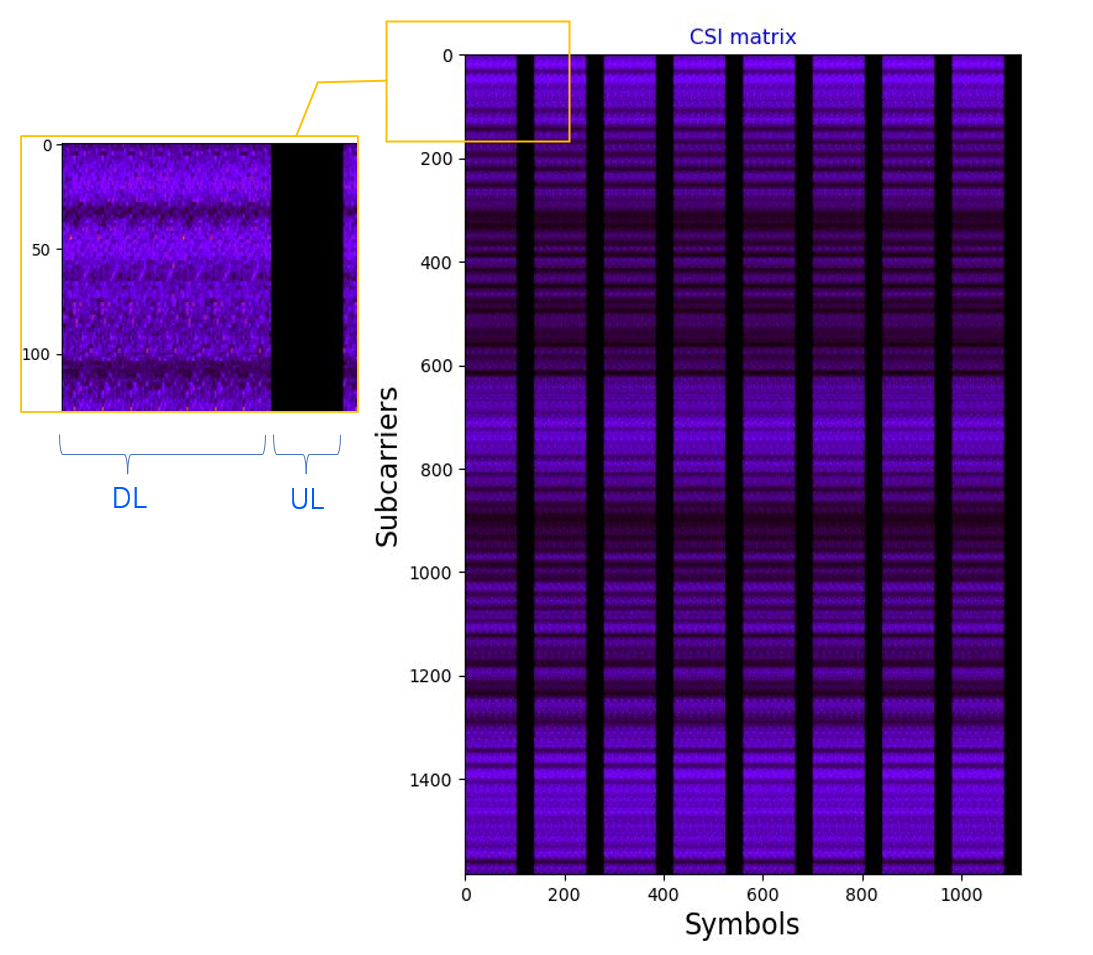
\includegraphics[width=0.5\textwidth]{Images/TDDprocessing/CSIMatrix_DLULpattern.png}
	    \caption{CSI matrix from Nokia PoC, rows and columns correspond to OFDM subcarriers and symbols, respectively}
	    \label{fig:CSIMatrix_DLULpattern}
	\end{figure}
	
	Received \gls{ul} symbols are transmitted from the \glspl{ue} towards the \gls{gnb} and are not generated by reflection of the \gls{dl} signal on objects in the environment.
	For this reason, they do not contain any useful information for radar processing, hence they are discarded (set to zero) before computing the periodogram.
    The removal of \gls{ul} symbols acts as windowing on the received frame. This introduces additional spectral replicas in the speed domain as shown in Figure \ref{fig:SpectralReplicasDLULpattern}. Replicas seem to appear at a constant speed displacement from where actual targets lie, behaving similarly to replicas introduced by the radar's non-ambiguity in speed.
    
    \begin{figure}[H]
        \centering
        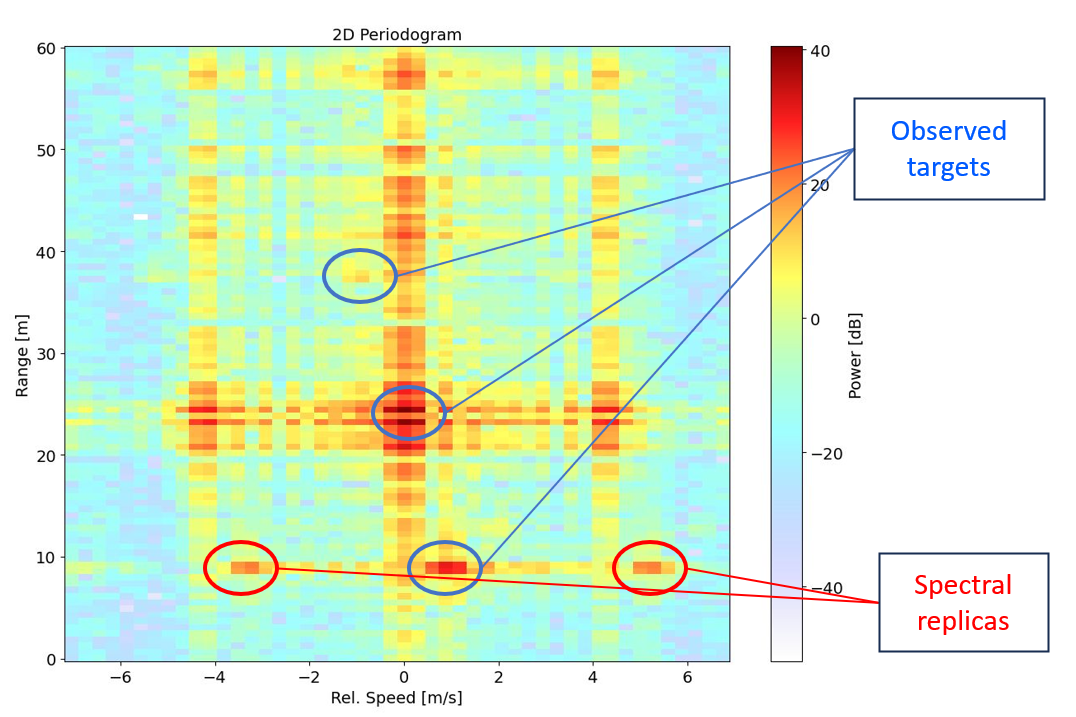
\includegraphics[width=0.55\textwidth]{Images/TDDprocessing/SpectralReplicasDLULpattern.png}
        \caption{Periodogram of a radar measurement with: static target at 23 m; moving target (range = 9,5 m, speed = 0.94 m/s); NLOS target (range = 37.2 m, speed = -1 m/s)}
        \label{fig:SpectralReplicasDLULpattern}
    \end{figure}
    
    In order to characterize the additional spectral replicas, the windowing function used to set all \gls{ul} symbols to zero is analyzed. The windowing pattern can be expressed in the form
    
    \begin{align}
        &\text{rect}\left( \frac{t + \tau}{104 \cdot T_S}\right) \ast \sum_{i=0}^7 \delta\left( t - i\cdot \frac{140}{1120}\cdot T_{\text{frame}} \right),  \\
        &T_{\text{frame}} = 1120 \cdot T_S.
    \end{align}

    The windowing function, apart from a time-shift factor, is a rectangle function (Dirichlet window) convoluted with a train of Dirac deltas with spacing of 140 samples, as shown in Figure \ref{fig:TDDproc_rectfunct}. Its frequency transform in Figure \ref{fig:TDDproc_rectfunct_transform}, is a cardinal sine (Dirichlet's kernel) function multiplied by a train of Dirac deltas.

    The transform is then convoluted with the signal in the frequency domain. The impulses adjacent to the one at zero-frequency appear as replicas in the periodogram. These peaks have sufficient power to be detected as real targets, thus limiting the performance of the system by reducing the effective unambiguous velocity. Even though their power is significantly lower compared to the main lobe, they can cause masking of real targets that would be detected near the replica, especially in \gls{nlos} where the return power is low. 

	\begin{figure}[H]
	    \centering
	    
	    \subfloat[TDD windowing function.\label{fig:TDDproc_rectfunct}]{%
	        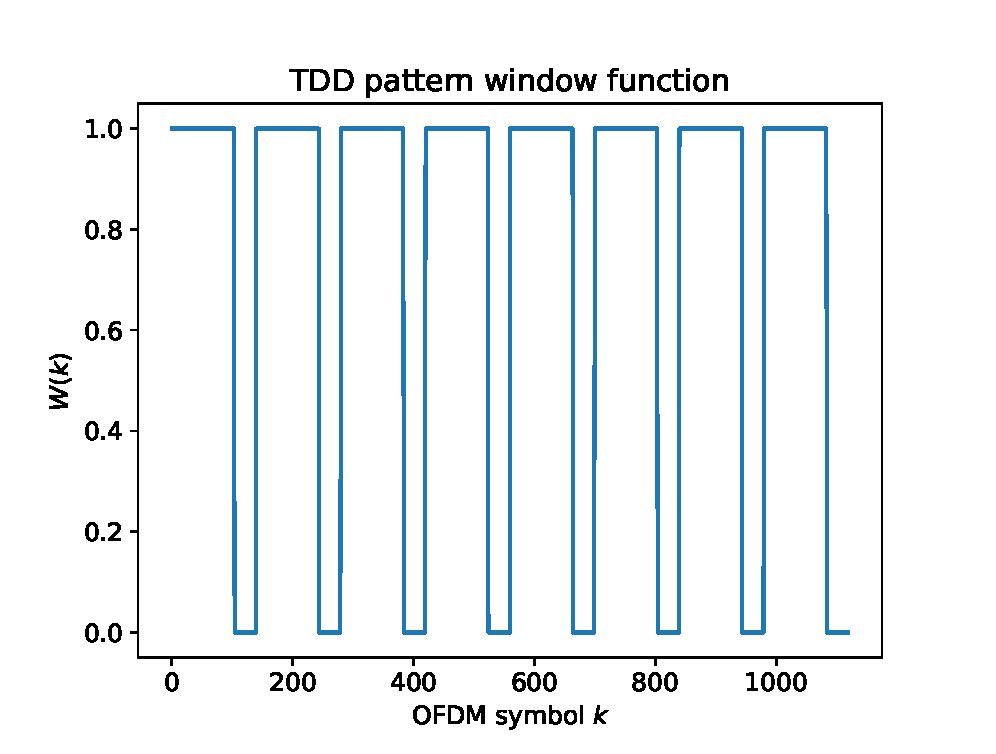
\includegraphics[scale=0.49]{Images/TDDprocessing/TDD_win.eps}%
	    }\hfill
	    \subfloat[Periodogram of the windowing function, FFT over 2048 points.\label{fig:TDDproc_rectfunct_transform}]{%
	        %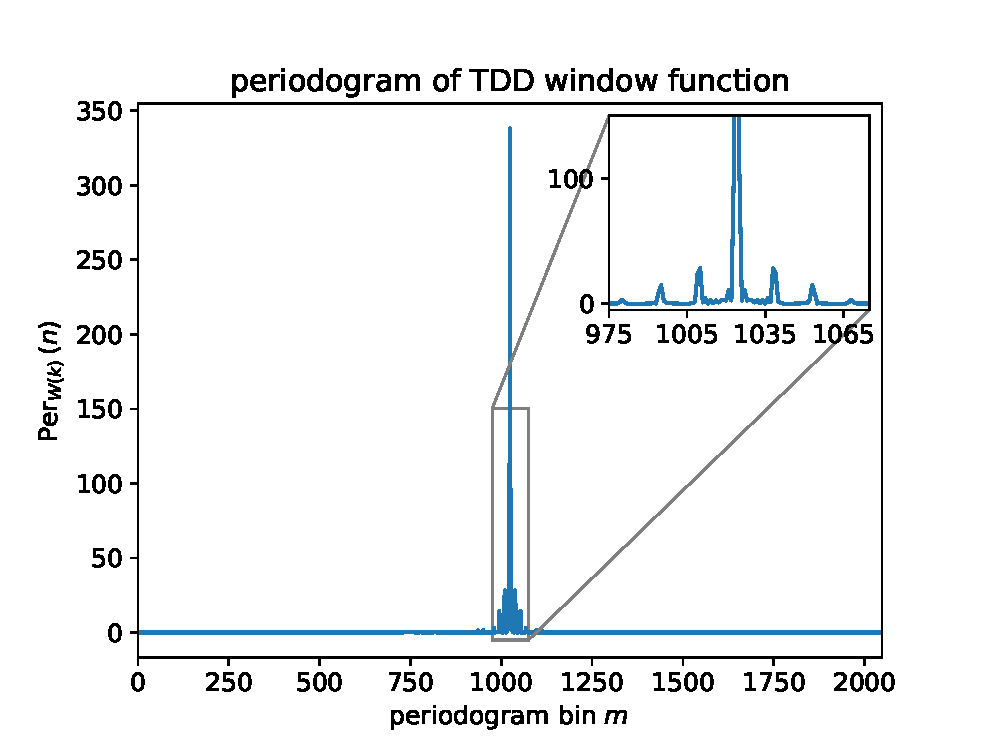
\includegraphics[scale=0.49]{Images/TDDprocessing/periodogram_of_TDD_win.eps}%
	        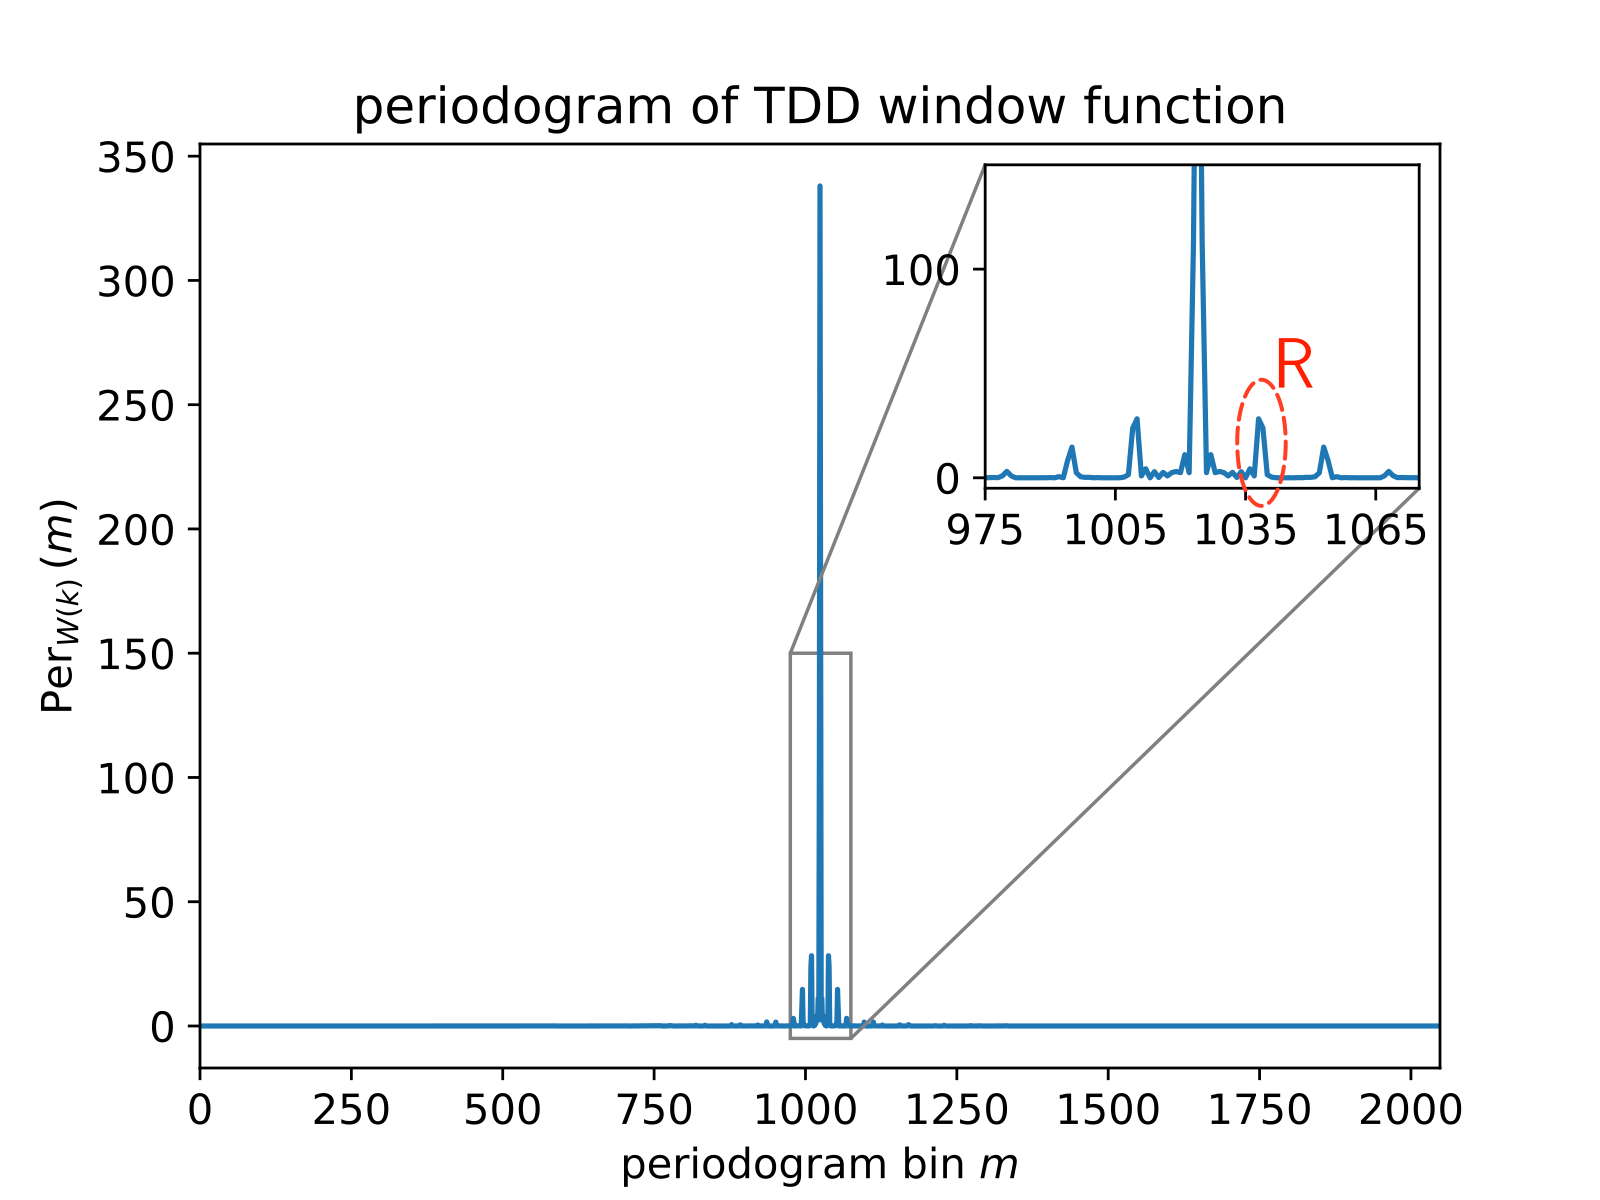
\includegraphics[scale=0.483]{Images/TDDprocessing/periodogram_of_TDD_win1.png}
	    }
	    
	    \caption[]{Representation of the time-windowing function applied to the \gls{csi} matrix. Sidelobe detected as replica is highlighted in red.}
	    \label{fig:TDDwindowingfunct}
	\end{figure}

	\subsection{PoC's fundamental performance limits}
		
		System performance can be evaluated in terms of resolution and unambiguous aperture, for both range and speed.
		Unambiguous range $d_{\text{unamb}}$ and speed $v_{\text{unamb}}$ are the maximum values that can be measured for a target without any ambiguity or ambiguity-related errors, and depend on the sampling rate in the respective domain, defined by subcarrier spacing and \gls{ofdm} symbol time.
		Range and speed resolution, $d_{\text{res}}$ and $v_{\text{res}}$, refer to the system's ability to resolve targets in terms of their range and speed and depend on the aperture in frequency and time domain, given by the overall bandwidth $\Delta f N$ and the frame duration $T_S M$, respectively. 
	
		When generating the periodogram by processing the \gls{csi} of a single frame, with the parameters indicated in Table \ref{table:PoCparams},
		the \gls{poc} operates with the following performance:
		
		\begin{itemize}
			\item \textbf{Unambiguous speed}
			\vspace{-\baselineskip} % Remove extra whitespace
			\begin{equation}
				v_{\text{unamb}} = \frac{c_0}{2f_C T_S} = 613.5\text{ m/s}.
			\end{equation}
			
			\item \textbf{Unambiguous range}
			\begin{equation}
				d_{\text{unamb}} = \frac{c_0}{2\Delta f} = 1250.0\text{ m}.
			\end{equation}
			\item \textbf{Speed resolution}
			\begin{equation}
				v_{\text{res}} = \frac{c_0}{2T_Sf_CM} = 0.547 \text{ m/s}.
			\end{equation} 
			\item \textbf{Range resolution}
			\begin{equation}
				d_{\text{res}} = \frac{c_0}{2\Delta fN} = 0.789 \text{ m}.
			\end{equation}  
		\end{itemize}
			This performance, especially the unambiguous speed, is more than sufficient for most indoor use cases. 
			This offers the possibility of applying different pre-processing strategies to the OFDM frame to avoid the presence of replicas. 
			As the TDD pattern acts on the time axis of the \gls{csi}, changing the time aperture or the \gls{ofdm} symbol rate will result in a change in speed resolution and unambiguous speed, respectively.
			Unambiguous speed is related with the time between two consecutive OFDM symbols. The distance between two consecutive processed symbols cannot be reduced without modifying the system parameters, but it can be increased by discarding some symbols, which worsens the unambiguity performance of the system.
			
			The next section analyses a number of possible strategies and their impact on system performance and their tradeoffs.    

	\subsection{Frame sampling strategies}

		    \begin{figure}[H]
		        \centering
		        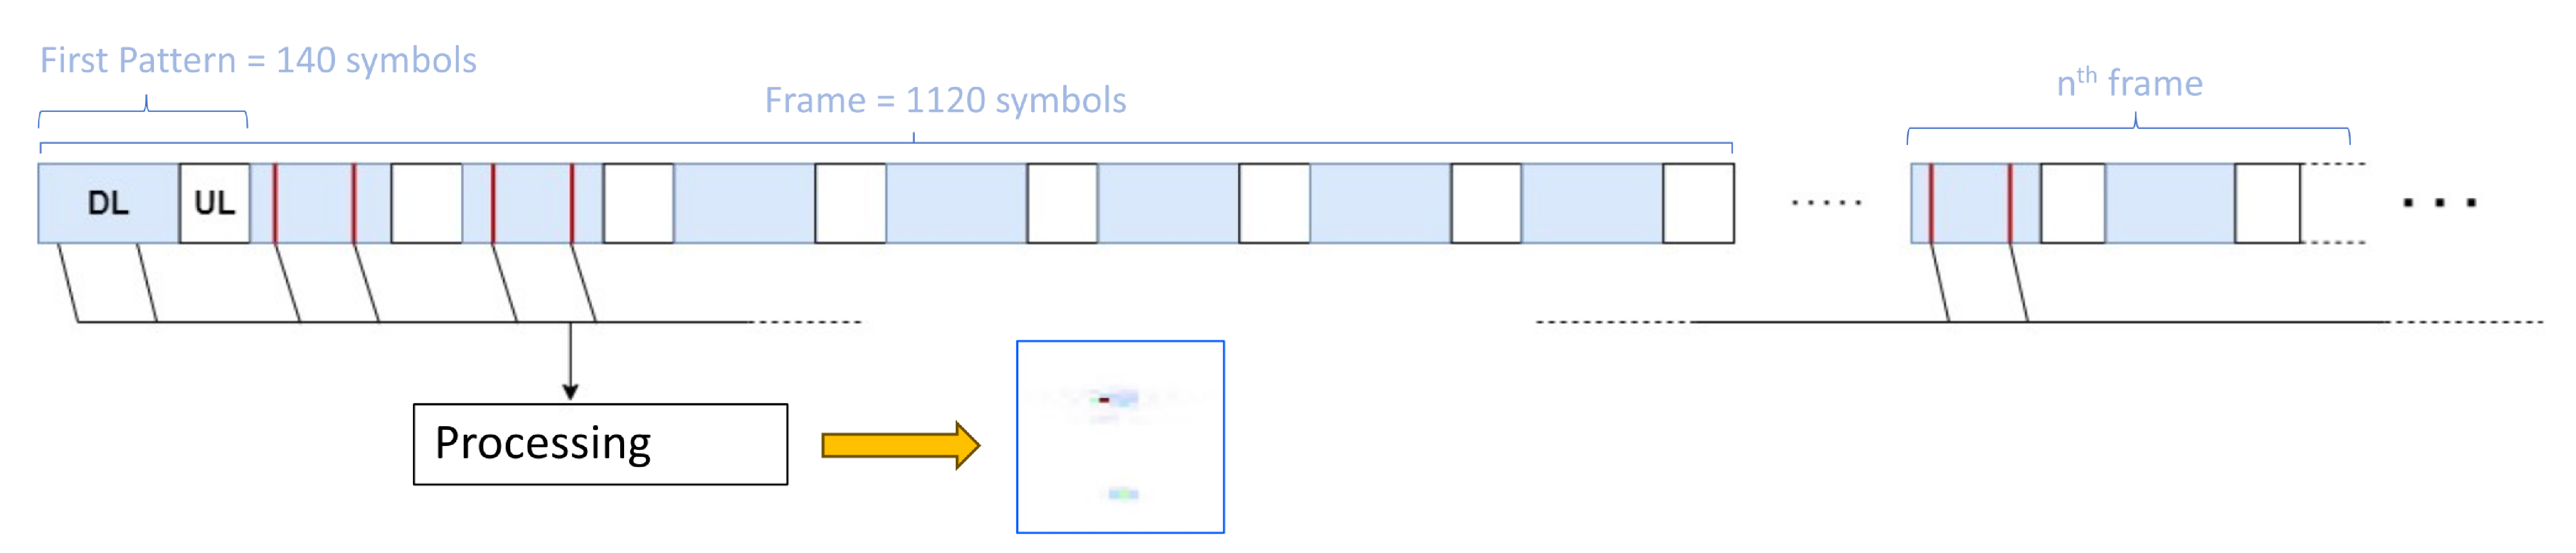
\includegraphics[width=1\textwidth]{Images/TDDprocessing/TDDstrategies.eps}
		        \caption{Decimation and combining of different consecutive frames}
		        \label{fig:TDDstrategies}
		    \end{figure}
		
		    \paragraph{Single DL pattern:}
		    to avoid processing empty \gls{ul} symbols, the simplest approach would be to process only the first 104 \gls{dl} symbols. The replicas would be avoided, but the time aperture of the measurement would be reduced more than eight times, worsening the speed resolution from $0.603$ m/s to approximately $5.88$ m/s, which is unusable for most indoor sensing use cases.
		    
		    \paragraph{Decimation at constant interval:}
		     a possible strategy is decimating the OFDM frame in time at a fixed pace, while avoiding blank \gls{ul} symbols. 
		     By discarding symbols, performance in unambiguous speed is reduced. However, by selecting symbols with a constant stride and avoiding \gls{ul} blanks, the windowing effect experienced by the standard frame is removed.
		     The minimum stride allowed for the single frame is one symbol every 47, which will select 3 symbols out of every \gls{dl} section.
		     
		     The overall amount of symbols in a processed \gls{csi} is reduced from 1120 to 24.
		     Replicas are not detected, but the lower number of processed elements results into a considerable loss of \gls{snr} in the periodogram. In the obtained measurements a loss of ca. 15 dB was detected, as shown in Figure \ref{fig:TDDperiodogram1FYesDec}. 
		     This affects \gls{nlos} sensing in particular, since targets observed from a reflection present a considerably lower peak power compared with the \gls{los} components.
		
		     Reducing the number of symbols available for sensing with a fixed time-aperture results in lower granularity of measurements and in a decrease in unambiguous speed. In the case of Figure \ref{fig:TDDperiodogram1FYesDec}, processing one symbol every 47, the obtained unambiguous speed is $13.05$ m/s. Speed resolution remains unchanged.
		    
		     \paragraph{Decimation and multi-frame processing:}
		     by combining consecutive frames, it is possible to process a higher number of symbols, regaining a part of the \gls{snr} thanks to processing gain, all without observing replicas. 
		     This also increases the time aperture of the measurement, resulting in better speed resolution.
		     
			 To combine several consecutive CSI measurements, the decimation rate is further reduced compared to the previous approach, from one sample in 47 to one sample every 70. 
			 Two symbols are chosen from each DL pattern, and UL symbols can be skipped across multiple consecutive frames.
			 The number of time samples obtained from a single CSI is reduced from 1120 to 16.
			 Unambiguous speed is also reduced further to $8.76$ m/s.
			 
			 To generate a radar update it is necessary to wait for multiple frames to be received.
			 This approach introduces a trade-off between \gls{snr} (processing gain) and update rate, with the update rate being reduced proportionally to the chosen time aperture.
		     For use cases such as intrusion detection, an update every 10 ms is not strictly necessary, and the higher detection probability due to the higher \gls{snr} is considered acceptable.
		          
		     To increase the number of updates, the observation time-window stride can be configured to be lower than its length, allowing for overlapping between processed time windows.
		      
		     Increasing the time aperture has two effects: it increases the speed resolution of the system and can result in migration effects, particularly for fast-moving targets. 
		     Range and speed migration occur when the target moves and changes velocity during the observation windows, resulting in a return "spread" in the obtained periodogram.
		     In the context of NLOS sensing, the impact of range migration on system performance is relatively low compared to the benefits of increased speed resolution and higher signal-to-noise ratio, as the primary objective is not to provide precise tracking or positioning data.
			
			Figures \ref{fig:TDDperiodogram1FNoDec}-\ref{fig:TDDperiodogram10frames} show the effects of the various strategies when applied to a OFDM radar measurement where both the \gls{nlos} and \gls{los} components are present for a single target.
			
		% 2x2 figure scheme
		    \begin{figure}[t]
		        \centering
		        
		        \subfloat[Standard processing, no decimation, SNR = 60.91 dB, \protect\newline $v_{\text{res}} = 0.603$ m/s, $ v_{\text{unamb}} = 613.15$ m/s
		\label{fig:TDDperiodogram1FNoDec}]{
		            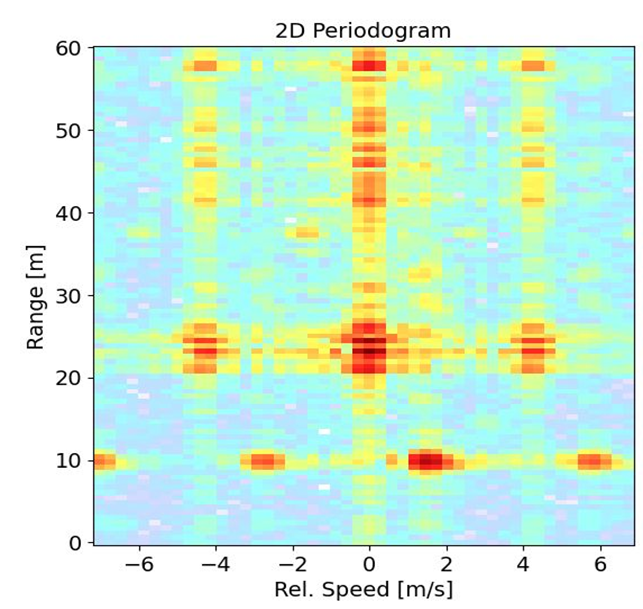
\includegraphics[width=0.4\textwidth]{Images/TDDprocessing/periodogram1FNoDec.png}
		        }
		        \hfill
		        \subfloat[CSI of single frame, decimated, \protect\newline SNR = 45.16 dB, \protect\newline $v_{\text{res}} = 0.603$ m/s, $ v_{\text{unamb}} = 13.05$ m/s\label{fig:TDDperiodogram1FYesDec}]{
		            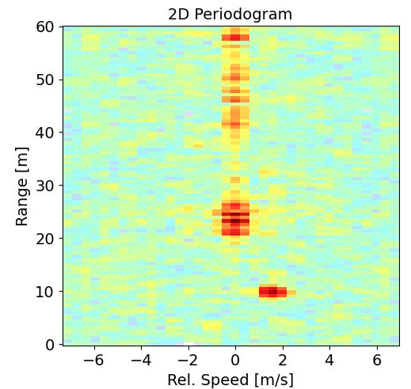
\includegraphics[width=0.4\textwidth]{Images/TDDprocessing/periodogram1FYesDec.png}
		        }
		        
		        \vspace{0.5cm}
		        
		        \subfloat[CSI of 6 processed frames, decimated, combined, SNR = 52.35 dB, \protect\newline $v_{\text{res}} = 0.091$ m/s, $ v_{\text{unamb}} = 8.76$ m/s\label{fig:TDDperiodogram6frames}]{
		            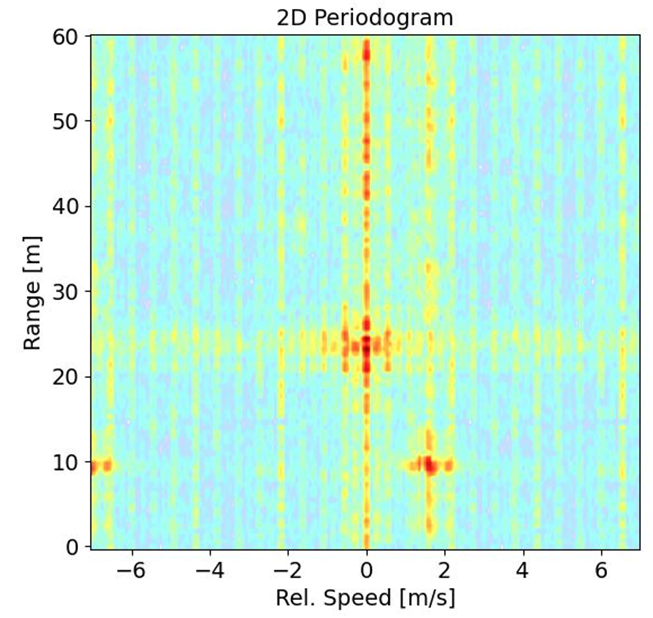
\includegraphics[width=0.4\textwidth]{Images/TDDprocessing/periodogram6frames.png}
		        }
		        \hfill
		        \subfloat[CSI of 10 processed frames, decimated, combined, SNR = 54.66 dB, \protect\newline $v_{\text{res}} = 0.054$ m/s, $ v_{\text{unamb}} = 8.76$ m/s\label{fig:TDDperiodogram10frames}]{
		            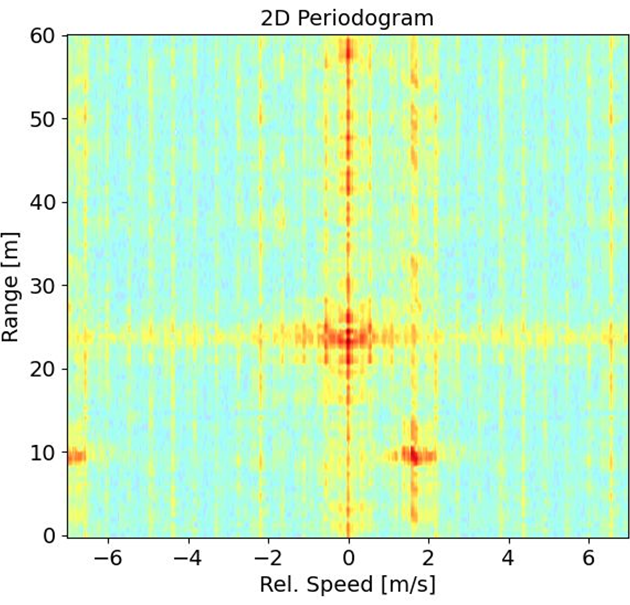
\includegraphics[width=0.4\textwidth]{Images/TDDprocessing/periodogram10frames.png}
		        }
		        
		        \caption{Examples of possible decimation and combining approaches in periodogram processing}
		        \label{fig:allperiodogram-decimation}
		    \end{figure}
		
		    
		
		
		    
		\begin{table}[H]
		    %\caption*{\textbf{Title of Table (optional)}}
		    \centering 
		    \caption{Comparison between SNR levels for different frame processing strategies}
		    \label{table:TDDstratcomparison}
		    \begin{tabular}{|p{9em} c c c |}
		    \hline
		    \rowcolor{bluepoli!40} % comment this line to remove the color
		    \textbf{Strategy} & \textbf{SNR [dB]} & \textbf{\textit{M}} & \textbf{Time aperture [ms]} \T\B \\
		    \hline \hline
		    $\textbf{Standard frame}$ & 60.91 & 1120 & 10 \T\B \\
		    $\textbf{Decimated frame}$ & 45.16 & 24 & 10 \T\B\\
		    $\textbf{6 frames}$ & 52.35 & 96 & 60  \T\B\\
		    $\textbf{10 frames}$ & 54.66 & 160 & 100  \T\B\\
		
		    \hline
		    \end{tabular}
		    \\
		\end{table}
		

	\subsection{Doppler artefacts observed for multiple frame processing}

		When processing several consecutive frames, Doppler artefacts can be observed in the corresponding periodograms.
		They appear as vertical lines of high power, compared to the underlying noise floor.
		For \gls{los} scenarios the artefacts do not limit the performance of the system, while their power is similar to the returns in \gls{nlos}.
		Figure \ref{fig:TDD_artefacts} shows that the power of the artefacts increases with the time aperture of the processed frame.
		The exact cause of these artefacts was not identified and their removal is out of the scope of this work. It is known that the 5G system used in the prototype from Nokia requires synchronization of component clock sources.
		It is likely that these artefacts are caused by phase compensations applied to the \gls{ofdm} signal both on a per-frame basis and within a single frame.
			\begin{figure}[H]
			\centering
			
			\subfloat[\footnotesize~Periodogram generated with 1 OFDM frame, decimated.\label{fig:artefacts1frame}]{%
				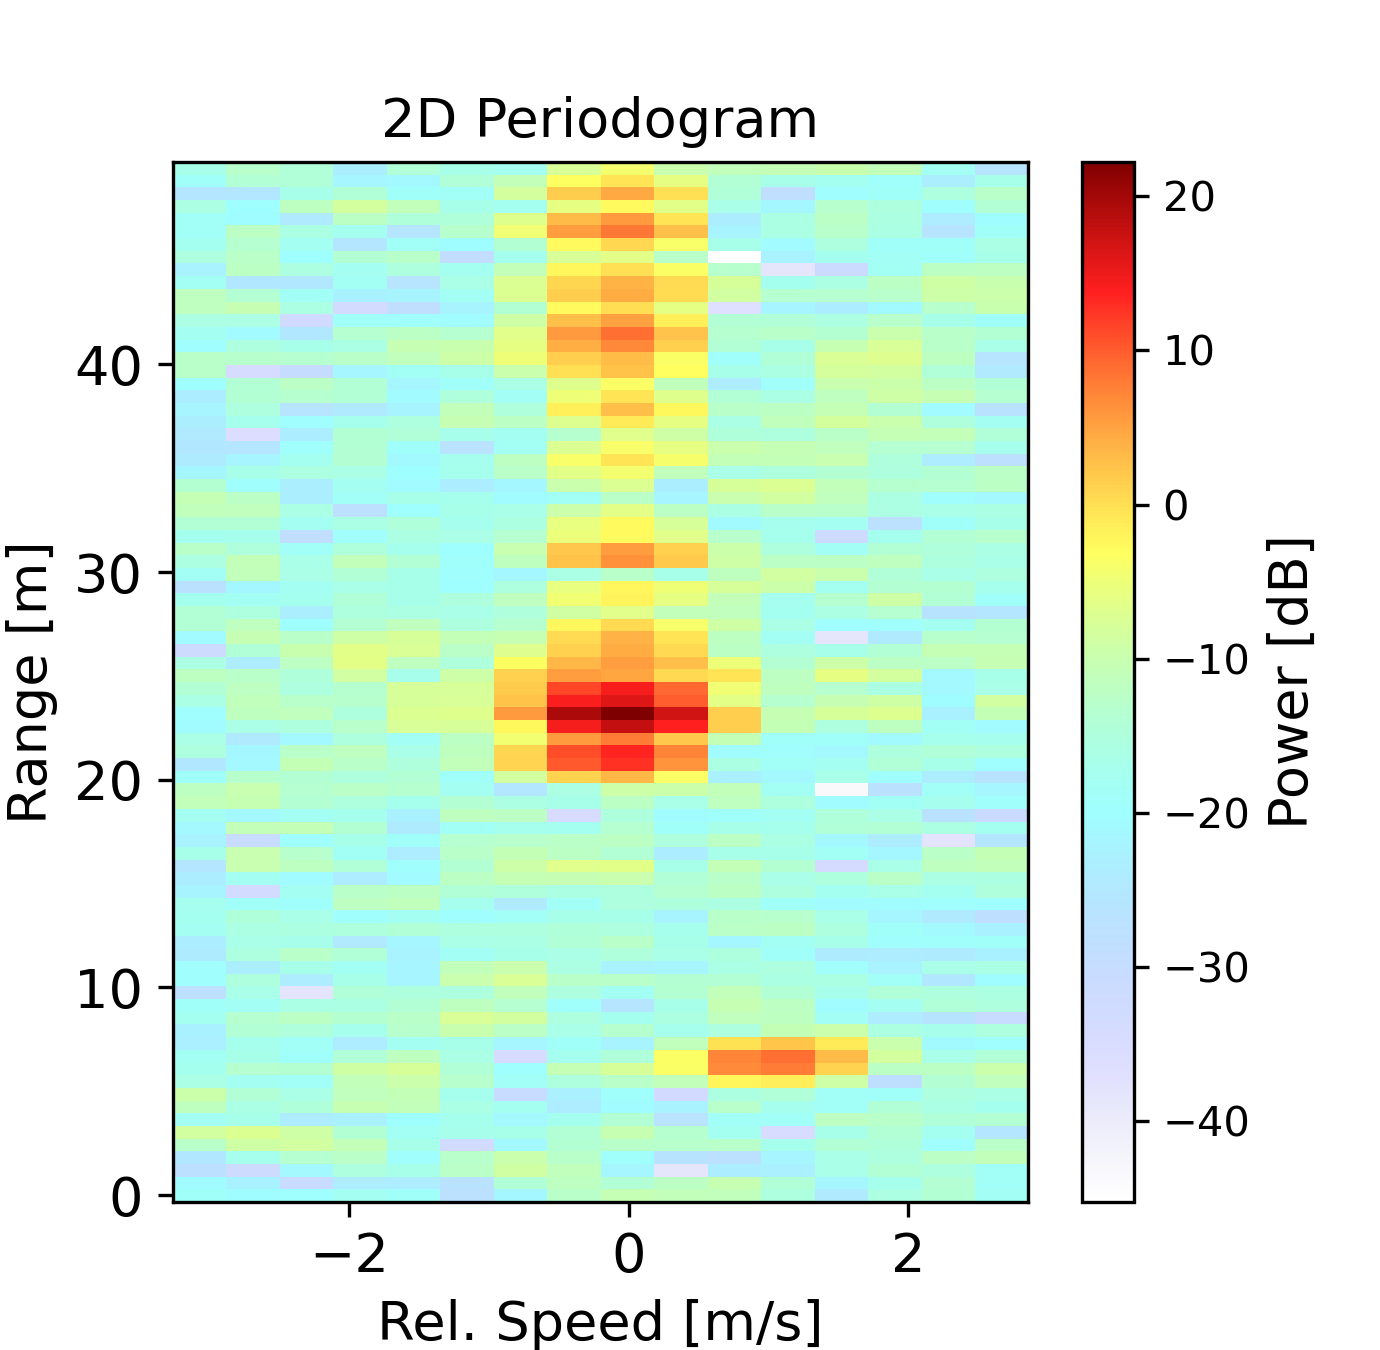
\includegraphics[scale=0.4]{Images/TDDprocessing/artefacts/1frames_periodogram.png}%
			}\hfill
			\subfloat[\footnotesize~Periodogram with\newline 2 OFDM frames, decimated.\label{fig:artefacts2frame}]{%
				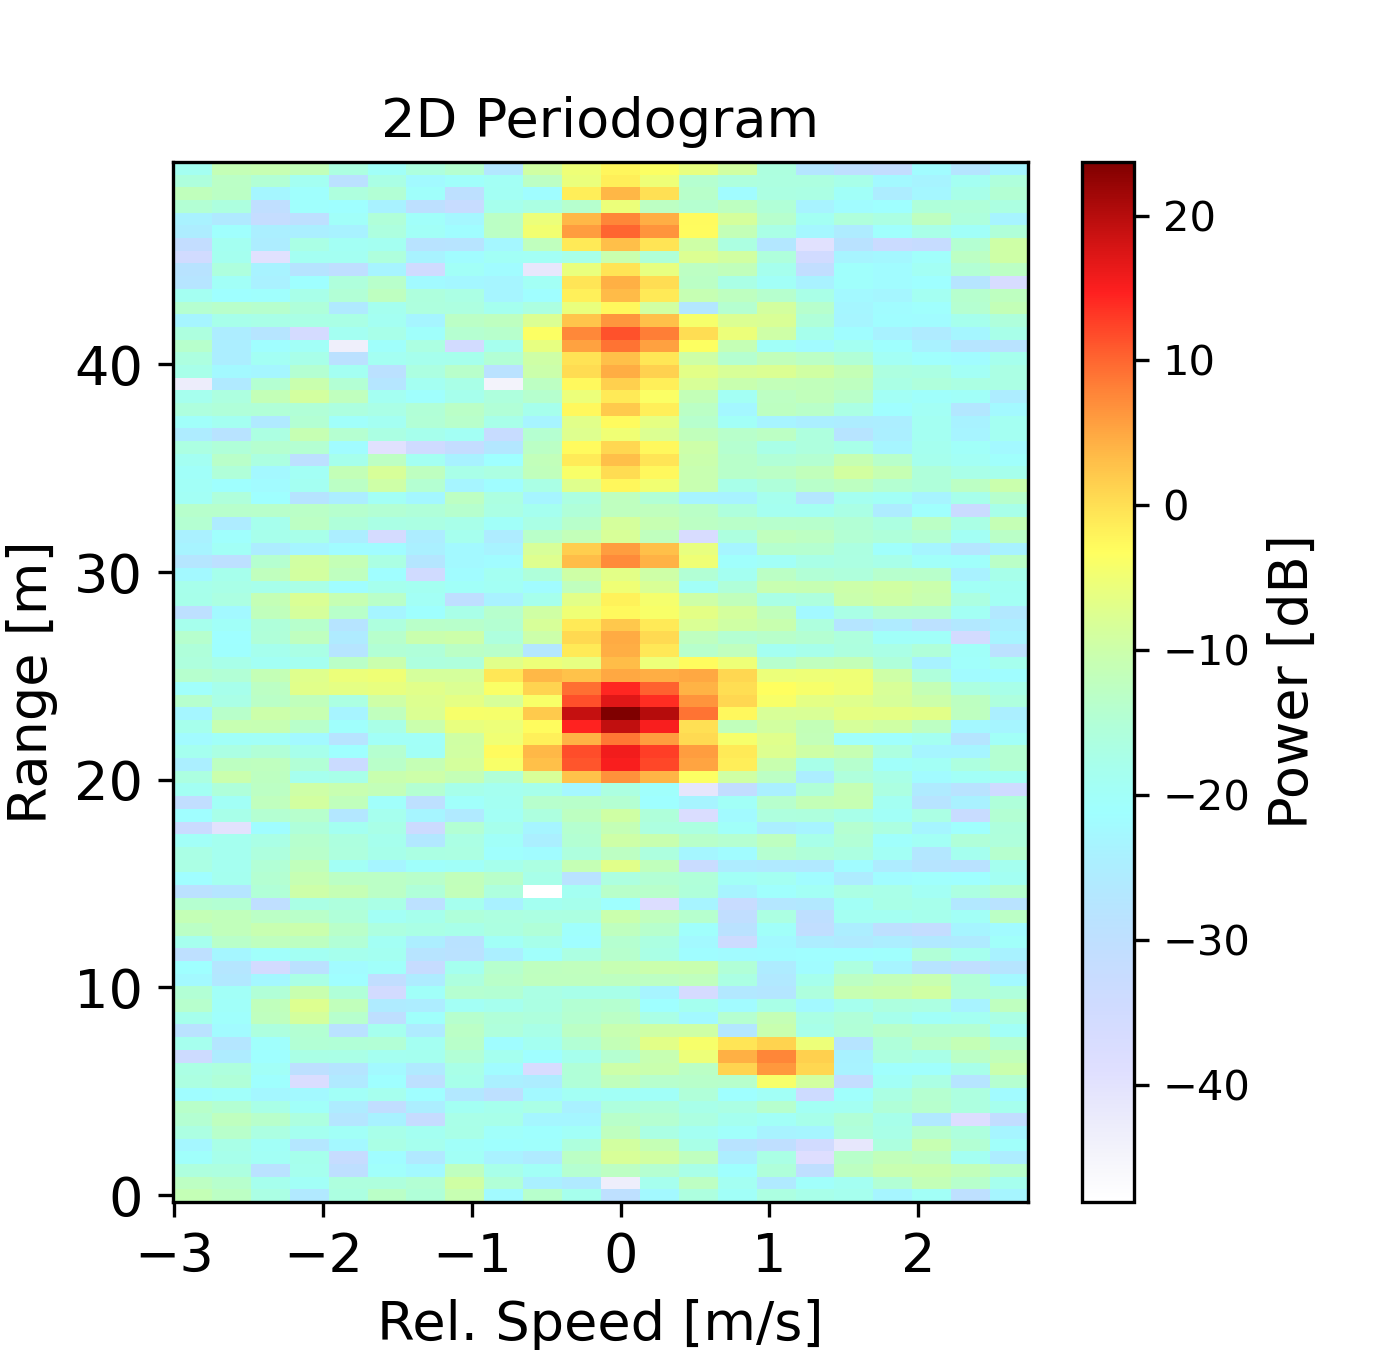
\includegraphics[scale=0.4]{Images/TDDprocessing/artefacts/2frames_periodogram.png}%
			}\hfill
			\subfloat[\footnotesize Periodogram with 3 OFDM frames, decimated.\label{fig:artefacts3frame}]{
				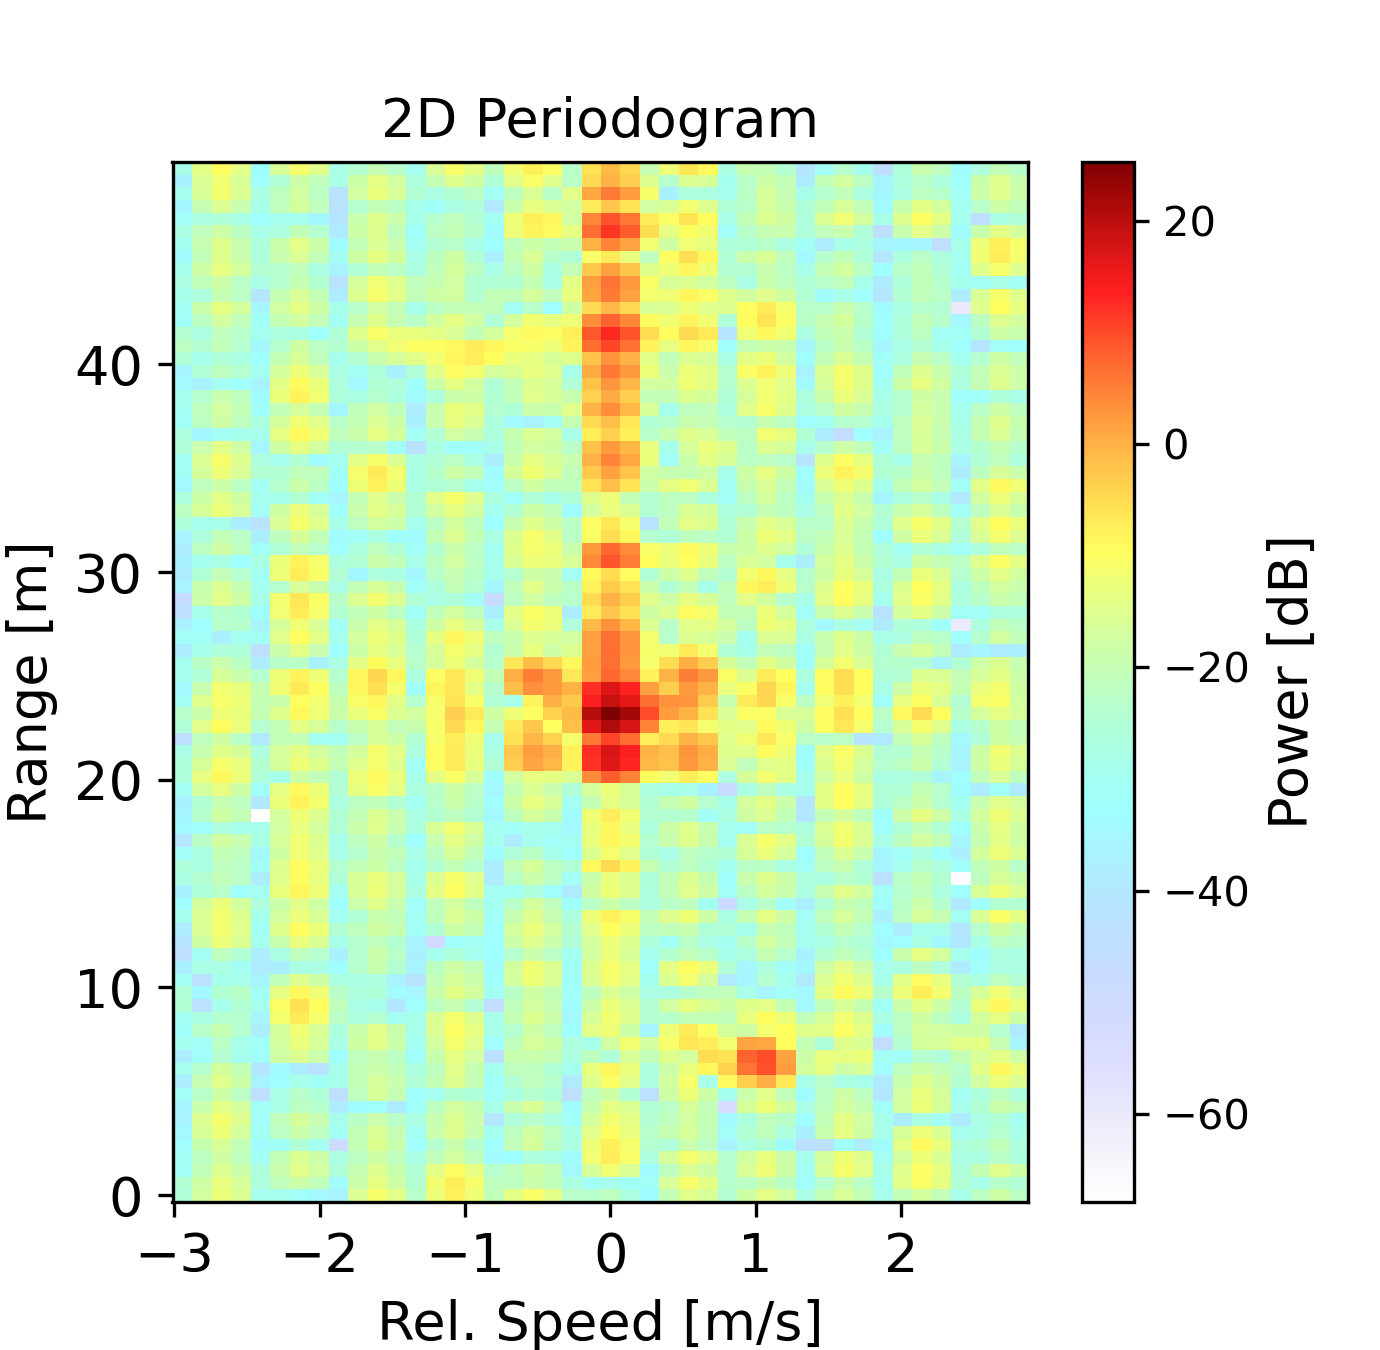
\includegraphics[scale=0.4]{Images/TDDprocessing/artefacts/3frames_periodogram.png}
			}\newline
			
			\subfloat[\footnotesize Periodogram with\newline 4 OFDM frames, decimated.\label{fig:artefacts4frame}]{%
				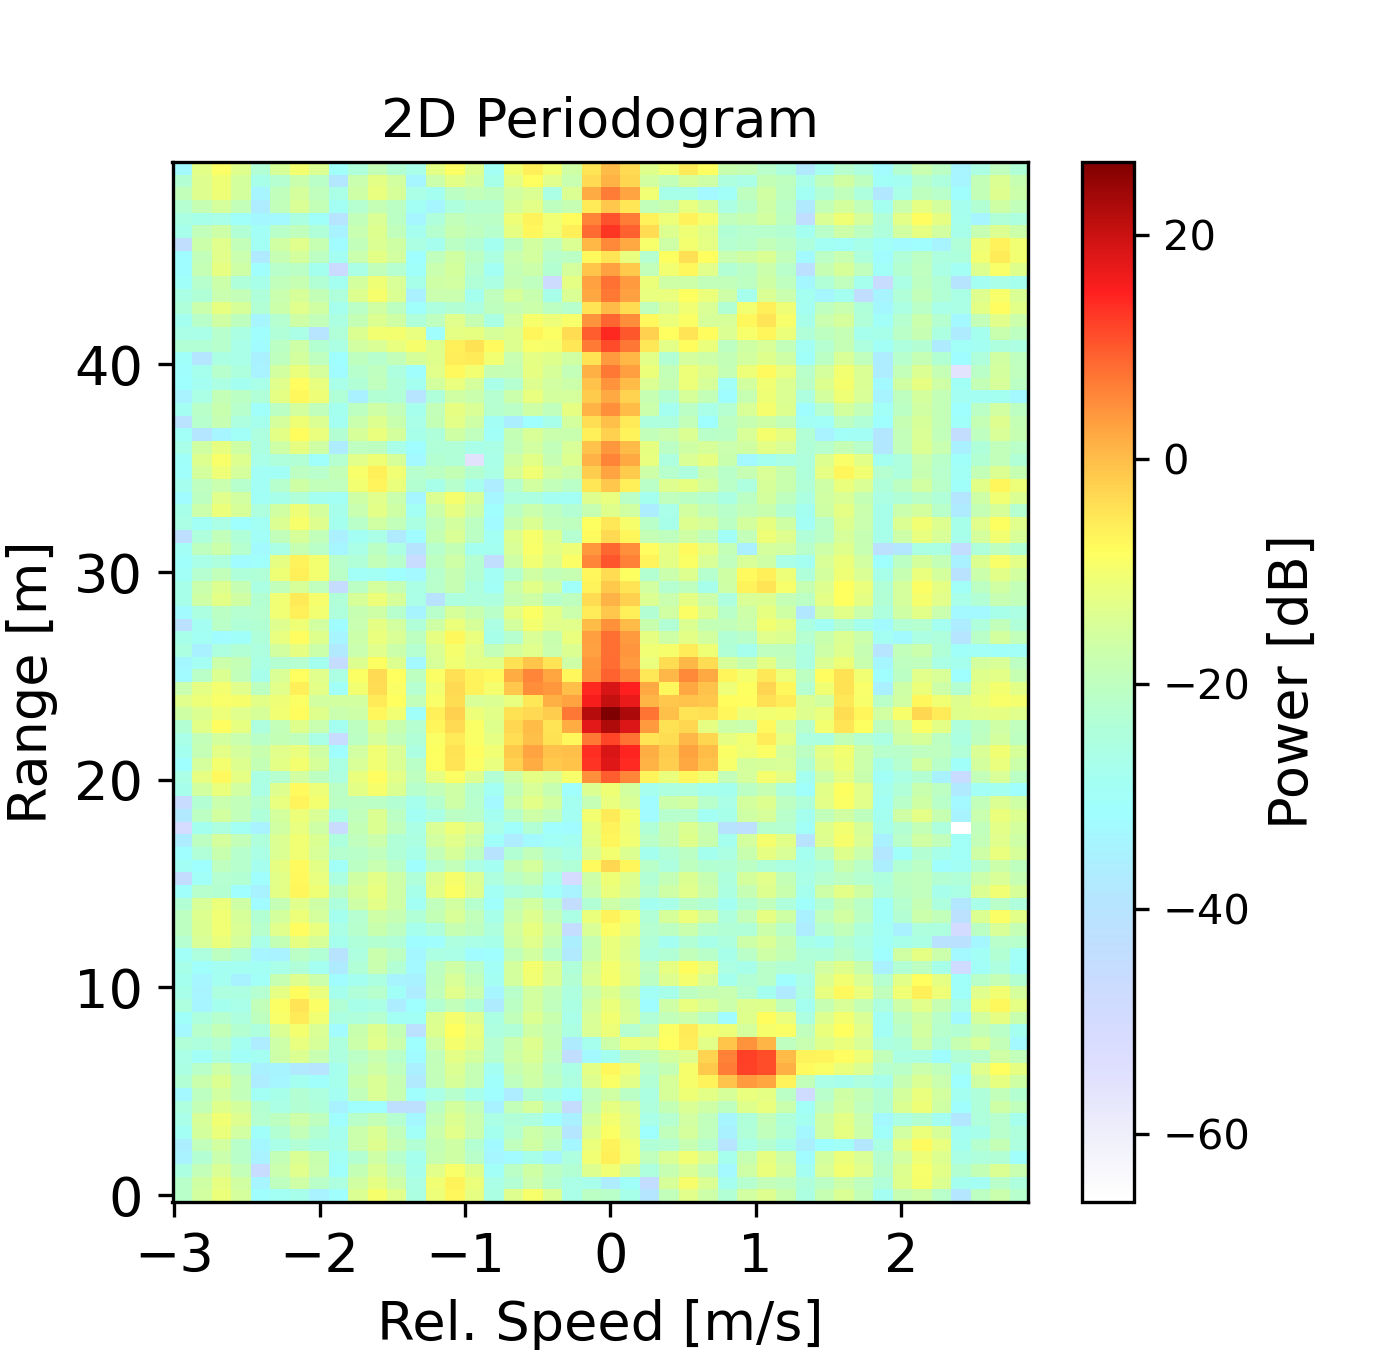
\includegraphics[scale=0.4]{Images/TDDprocessing/artefacts/4frames_periodogram.png}%
			}\hfill
			\subfloat[\footnotesize Periodogram with 5 OFDM frames, decimated.\label{fig:artefacts5frame}]{%
				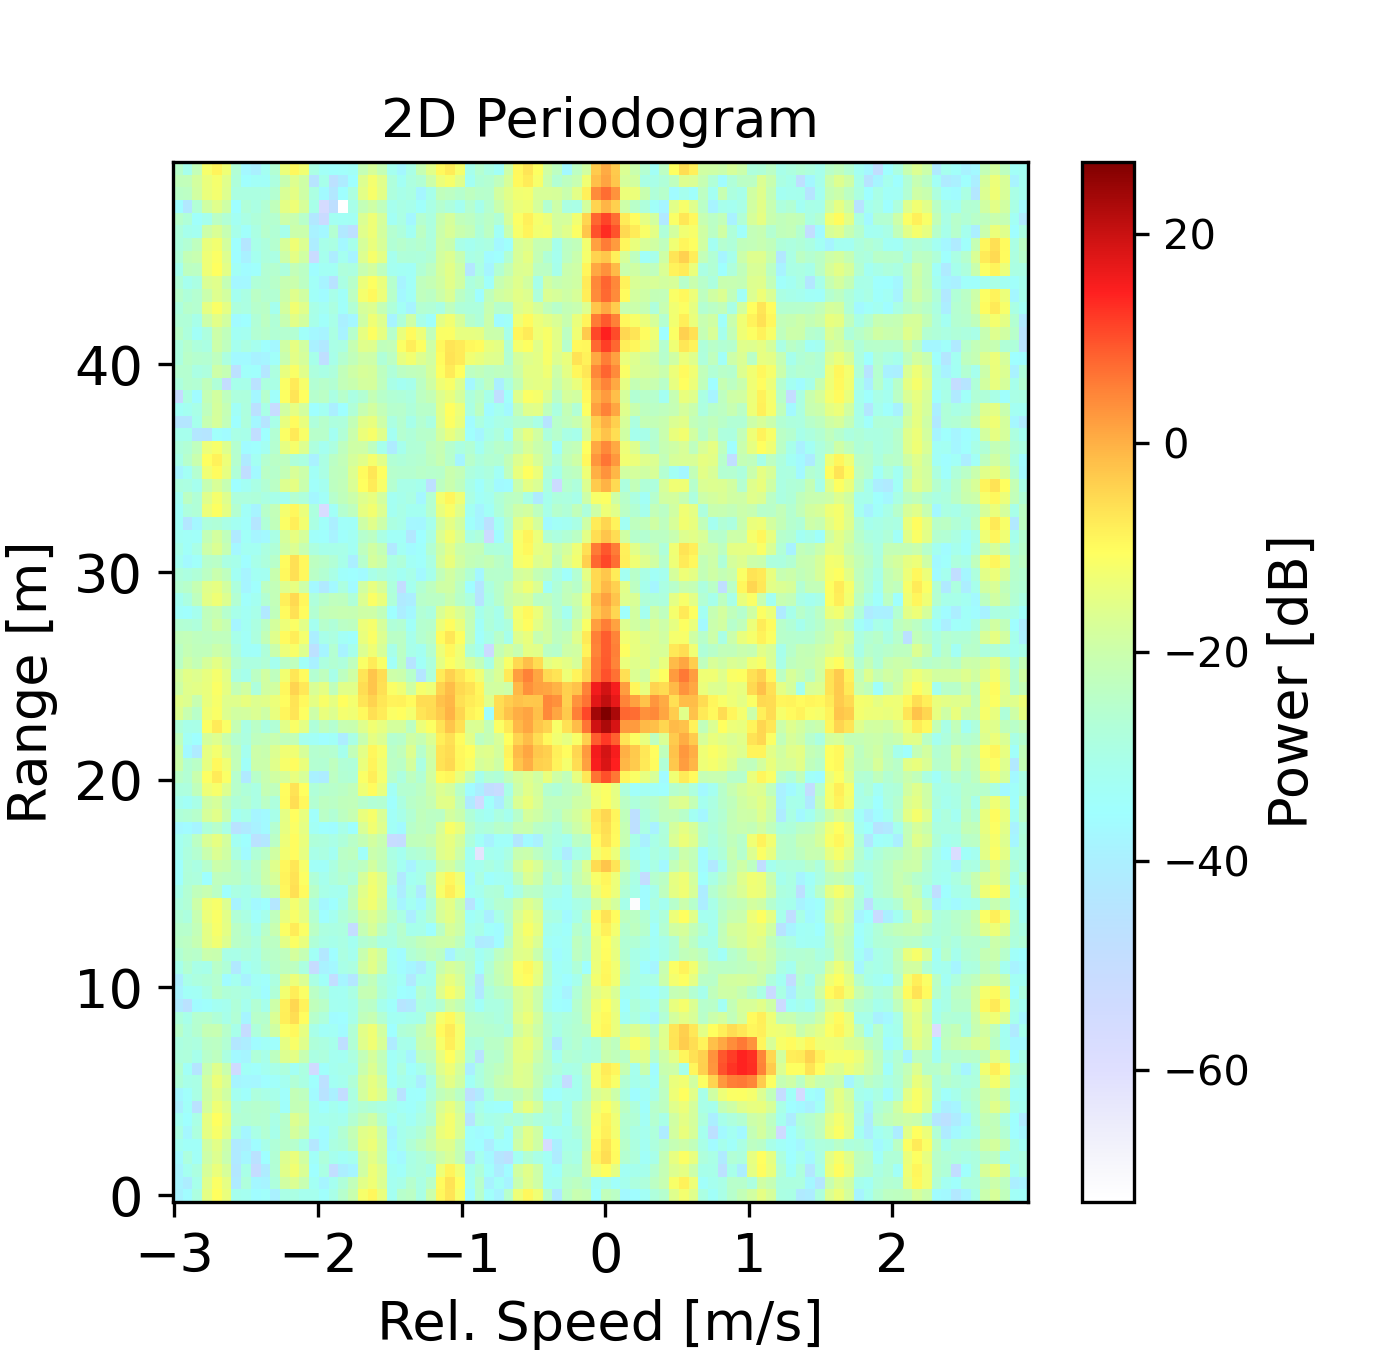
\includegraphics[scale=0.4]{Images/TDDprocessing/artefacts/5frames_periodogram.png}%
			}\hfill
			\subfloat[\footnotesize Periodogram with 6 OFDM frames, decimated. \label{fig:artefacts6frame}]{%
				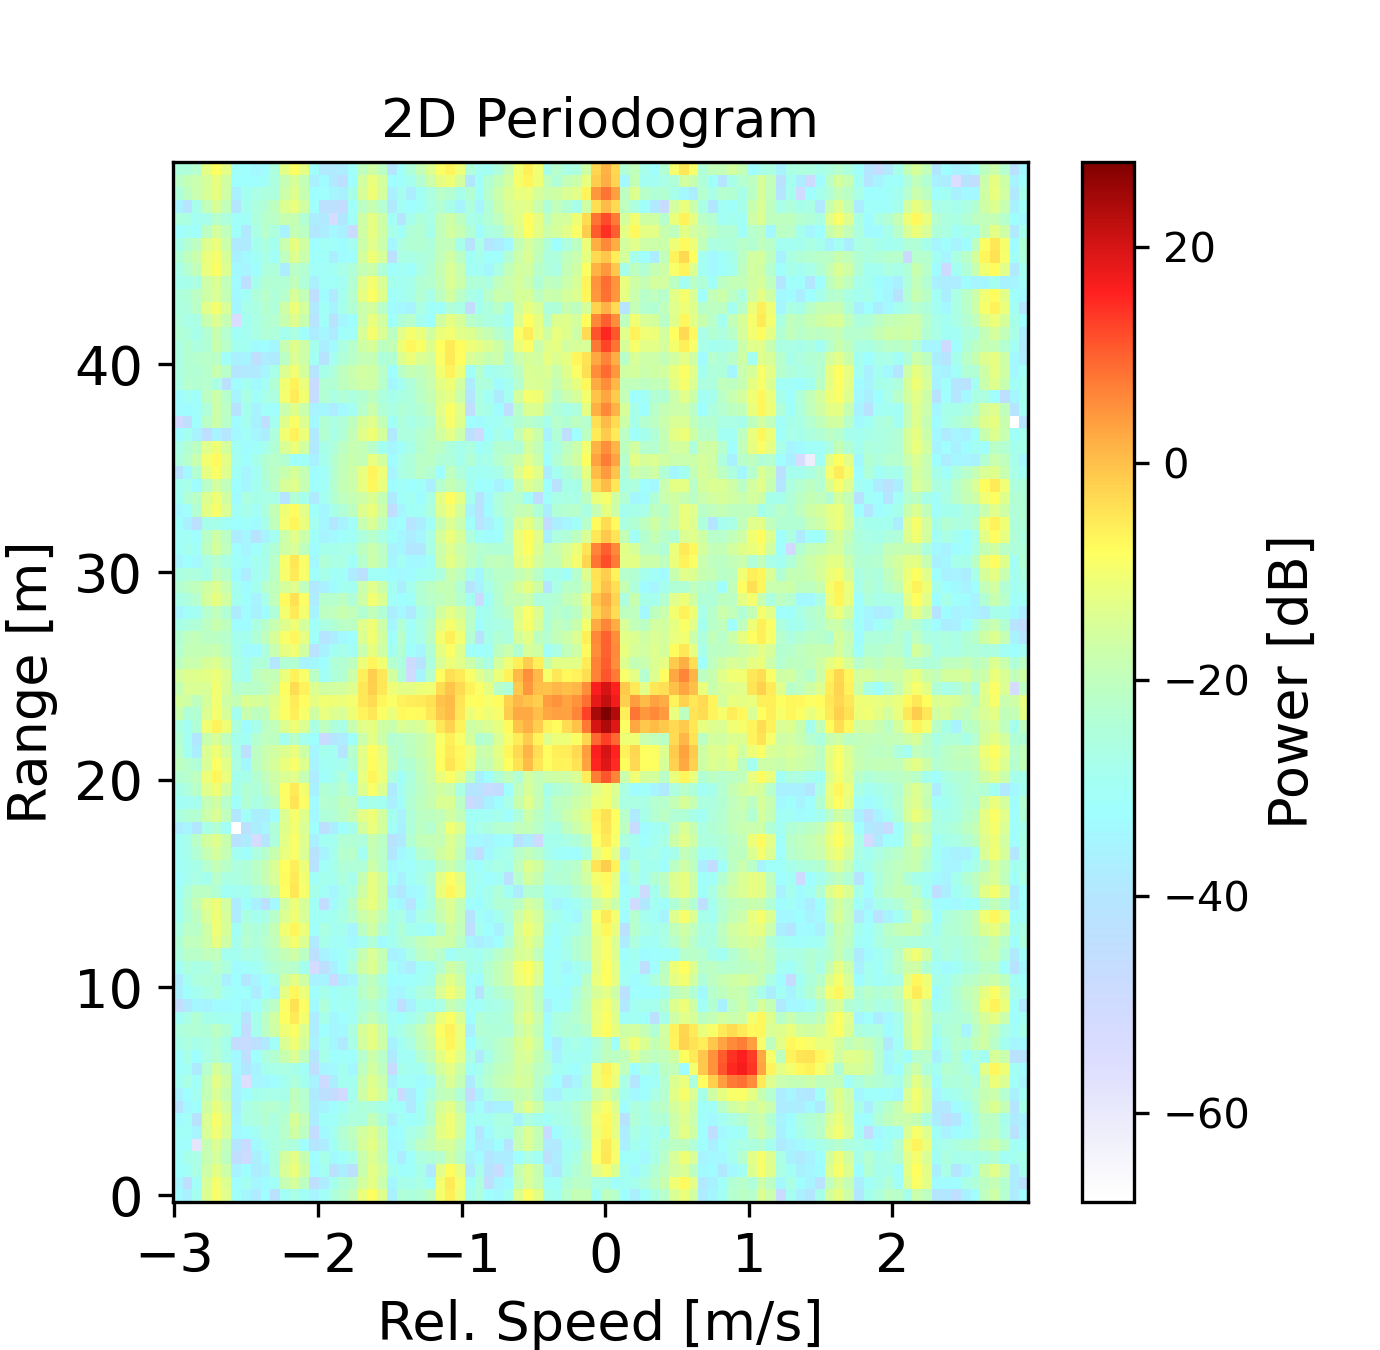
\includegraphics[scale=0.4]{Images/TDDprocessing/artefacts/6frames_periodogram.png}%
			}
			\caption[]{\small Comparison of periodograms from sensing acquisitions obtained in NOKIA's industrial test facility.
				Periodogram are generated from the same measurement data. When using a single OFDM frame the periodogram is sampled selecting one symbol every 47, whilst one every 70 is kept in the other cases using multiple frames.  }
			\label{fig:TDD_artefacts}
		\end{figure}
		
		